\chapter{Examples}\label{chap:chap}

\keywords{Word 4, Word 5, Word 6}

% TODO add sections depths and references to them
\section{Section}\label{sec:sec}
\subsection{SubSection}\label{subsec:subsec}
\subsubsection{SubSubSection}\label{subsubsec:subsubsec}
\paragraph{Paragraph}\label{par:par}
\subparagraph{SubParagraph}\label{subpar:subpar}


\section{Citations \& References (plus lists)}

Example bulleted list, of example cross references:
\begin{itemize}
    \item Example citation \cite{smit54}
    \item Example multi-citation \cite{smit54,colu92}
    \item Example multi-citation \cite{smit54,colu92,gree00}
    \item Example cross reference \cref{examples:figures}
    \item Example cross references \cref{chap:chap,sec:sec,subsec:subsec,subsubsec:subsubsec,par:par,subpar:subpar}
    \item Example figure reference \cref{fig:referenceToFigure1}
    \item Example sub-figure reference \cref{fig:referenceToFigure1a}
    \item Example multi-figure reference \cref{fig:referenceToFigure1,fig:referenceToFigure2,fig:expPlot}
    \item Example table reference \cref{tbl:referenceToTable1}
    \item Example equation reference \cref{eq:referenceToEq1}
    \item Example algorithm reference \cref{alg:referenceToAlg}
    \item Example term \gls{latex} or \Gls{latex}
    \item Example abbreviation first use \gls{gcd}
    \item Example abbreviation second use \gls{gcd}
    \item Example company and product \useproper{matlab} and \useproper{simulink} by \useproper{mathworks} 
    \item Example abbreviation, term, and organization all in one \gls{nasa@abbr}
    \item Example hyperlink \href{https://www.lipsum.com/}{Lorem Ipsum}
    \item[Note:] I would like to describe something here
    \item[Caveat!] And give a warning here
\end{itemize} ~


Example numbered list:
\begin{enumerate}
    \item \label{itm:first} First level item
    \item \label{itm:second} First level item
    \begin{enumerate}
        \item \label{itm:third} Second level item
        \item Second level item
        \begin{enumerate}
        \item Third level item
        \item Third level item
        \begin{enumerate}
            \item Fourth level item
            \item Fourth level item
        \end{enumerate}
        \end{enumerate}
    \end{enumerate}
\end{enumerate} ~

Take special note of \cref{itm:first,itm:second} and \cref{itm:third}.


\section{Figures} \label{examples:figures}

\begin{figure}[H]
    \centering
    \includegraphics[width=\textwidth]{./Helpers/blank.jpg}
    \caption{Caption information for figure} 
    \label{fig:referenceToFigure1}
\end{figure}

\begin{figure}[H]
    \centering

    \begin{subfigure}[b]{0.3\textwidth}
        \includegraphics[width=\textwidth]{./Helpers/blank.jpg}
         \caption{One} 
         \label{fig:referenceToFigure1a}
    \end{subfigure}
    ~
    \begin{subfigure}[b]{0.3\textwidth}
        \includegraphics[width=\textwidth]{./Helpers/blank.jpg}
        \caption{Two}
    \end{subfigure}
    ~
    \begin{subfigure}[b]{0.3\textwidth}
        \includegraphics[width=\textwidth]{./Helpers/blank.jpg}
         \caption{Three}
    \end{subfigure}
    \caption{Caption information for sub-figures} 
    \label{fig:referenceToFigure2}
\end{figure}


\section{Table}

\begin{table}[h]
	\centering
	\caption[Table info in LoT]{Full caption information}
	\label{tbl:referenceToTable1}
	\begin{tabularx}{0.5\textwidth}{X | c}
	\multicolumn{1}{c}{\textbf{Header1}} &  \multicolumn{1}{c}{\textbf{Header2}} \\ \hline
	  A1 & B1 \\
	  A2 & B2 \\
	  A3 & B3
	\end{tabularx}
\end{table}

\begin{table}[H]
	\caption{Pros and cons of ...}
	\label{tbl:referenceToTable2}
    \begin{tabularx}{\linewidth}{>{\parskip1ex}X@{\kern4\tabcolsep}>{\parskip1ex}X}
        \toprule
        \hfil\bfseries Pros
        &
        \hfil\bfseries Cons
        \\\cmidrule(r{3\tabcolsep}){1-1}\cmidrule(l{-\tabcolsep}){2-2}
        
        %% PROS, separated by empty line or \par
        Item \par
        
        &
        
        %% CONS, separated by empty line or \par
        Item \par
        
        \\\bottomrule
    \end{tabularx}
\end{table}


\section{Equation}

\begin{equation} 
    \label{eq:referenceToEq1}
	\begin{gathered}
		\min_\beta \sum_{i=1}^n \left( y_i - \sum_{j=1}^p \beta_j x_{ij} \right)^2 + \lambda_2 \sum_{j=1}^p \beta_j^2
	\end{gathered}
\end{equation}

\namedequation{a^2 + b^2 = c^2}{Pythagorean Theorem}{eq:referenceToEq2}


\section{Algorithms}

\begin{lstlisting}[language=Python, caption=Python example, label=alg:referenceToAlg]
import numpy as np
x = "test"
    
def incmatrix(genl1,genl2):
    m = len(genl1)
    n = len(genl2)
    M = None #to become the incidence matrix
    VT = np.zeros((n*m,1), int)  #dummy variable
    
    #compute the bitwise xor matrix
    M1 = bitxormatrix(genl1)
    M2 = np.triu(bitxormatrix(genl2),1) 

    for i in range(m-1):
        for j in range(i+1, m):
            [r,c] = np.where(M2 == M1[i,j])
            for k in range(len(r)):
                VT[(i)*n + r[k]] = 1;
                VT[(i)*n + c[k]] = 1;
                VT[(j)*n + r[k]] = 1;
                VT[(j)*n + c[k]] = 1;
                
                if M is None:
                    M = np.copy(VT)
                else:
                    M = np.concatenate((M, VT), 1)
                
                VT = np.zeros((n*m,1), int)
    
    return M
\end{lstlisting}


\section{Plots \& Flow Charts}

\begin{figure}[H]
    \center
    \begin{tikzpicture}
        \begin{axis}
            \addplot[color=red]{exp(x)};
        \end{axis}
    \end{tikzpicture}
    \caption{Example automatic exponential plot.} 
    \label{fig:expPlot}
\end{figure}

\begin{figure}[H]
    \center
    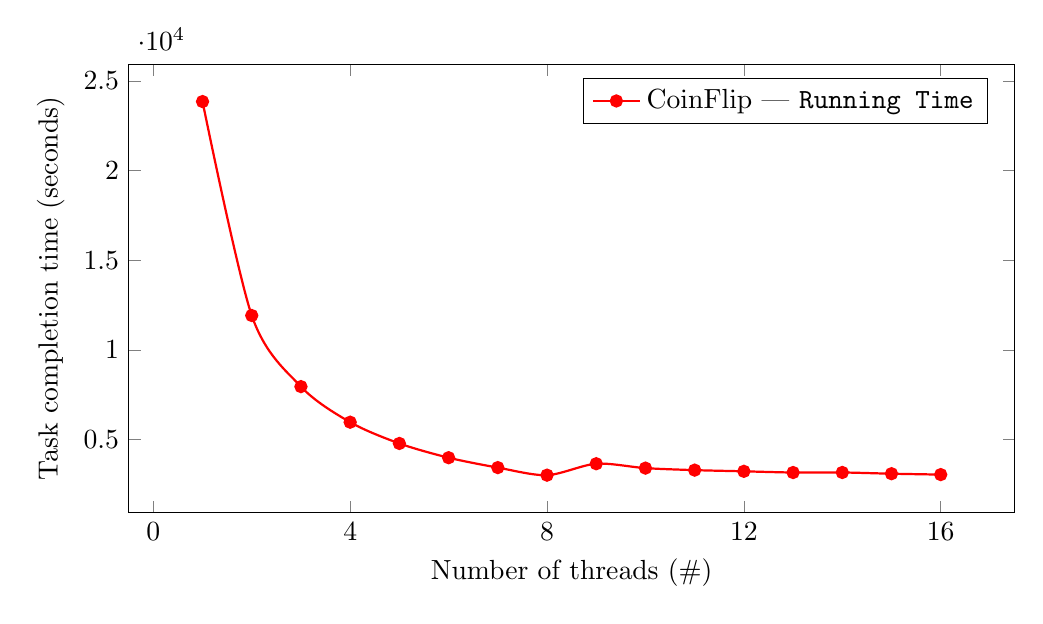
\begin{tikzpicture}
        \begin{axis}[
            xlabel = Number of threads (\#),
            ylabel = Task completion time (seconds),
            xtick = {0, 4, 8, 12, 16},
            ytick = {0, 5000, 10000, 15000, 20000, 25000},
            % ymax = 6,
            % ymin = 0,
            x = 2.5cm/4,
            legend pos = north east]

        \addplot[smooth, thick, color = red, mark = *]
            plot coordinates {
                (1, 23849)
                (2, 11920)
                (3, 7955.8)
                (4, 5971.6)
                (5, 4786.2)
                (6, 3991.8)
                (7, 3440.4)
                (8, 3018.4)
                (9, 3656.2)
                (10, 3411.2)
                (11, 3299)
                (12, 3233)
                (13, 3165.8)
                (14, 3168.2)
                (15, 3099.4)
                (16, 3050.4)
            };
        \addlegendentry{CoinFlip --- \texttt{Running Time}} 
        \end{axis}
    \end{tikzpicture}
    \caption{Example manual plot.} 
    \label{fig:manualPlot}
\end{figure}


% Flow chart styles
\tikzstyle{startstop} = [rectangle, rounded corners, 
minimum width=3cm, 
minimum height=1cm,
text centered, 
draw=black, 
fill=red!30]

\tikzstyle{io} = [trapezium, 
trapezium stretches=true, % A later addition
trapezium left angle=70, 
trapezium right angle=110, 
minimum width=3cm, 
minimum height=1cm, text centered, 
draw=black, fill=blue!30]

\tikzstyle{process} = [rectangle, 
minimum width=3cm, 
minimum height=1cm, 
text centered, 
text width=3cm, 
draw=black, 
fill=orange!30]

\tikzstyle{decision} = [diamond, 
minimum width=3cm, 
minimum height=1cm, 
text centered, 
draw=black, 
fill=green!30]
\tikzstyle{arrow} = [thick,->,>=stealth]

\begin{figure}[H]
    \centering
    \begin{singlespace}
        \begin{tikzpicture}[node distance=2cm]

            \node (start) [startstop] {Start};
            \node (in1) [io, below of=start] {Input};
            \node (pro1) [process, below of=in1] {Process 1};
            \node (dec1) [decision, below of=pro1, yshift=-0.5cm] {Decision 1};

            \node (pro2a) [process, below of=dec1, yshift=-0.5cm] {Process 2a \\
            text text text text  \\ 
            text text text};

            \node (pro2b) [process, right of=dec1, xshift=2cm] {Process 2b};
            \node (out1) [io, below of=pro2a] {Output};
            \node (stop) [startstop, below of=out1] {Stop};

            \draw [arrow] (start) -- (in1);
            \draw [arrow] (in1) -- (pro1);
            \draw [arrow] (pro1) -- (dec1);
            \draw [arrow] (dec1) -- node[anchor=east] {yes} (pro2a);
            \draw [arrow] (dec1) -- node[anchor=south] {no} (pro2b);
            \draw [arrow] (pro2b) |- (pro1);
            \draw [arrow] (pro2a) -- (out1);
            \draw [arrow] (out1) -- (stop);
            
        \end{tikzpicture}
    \end{singlespace}
    \caption{Example flow chart.} 
    \label{fig:flowChart}
\end{figure}


\closechapter
